\documentclass[11pt]{article}

\usepackage{graphicx}
\usepackage[top=25mm, bottom=25mm, left=25mm, right=25mm, a4paper]{geometry}
\usepackage{amsmath}
\usepackage{enumitem}
\usepackage{float}
\usepackage{fancyhdr}
\usepackage{booktabs}
\usepackage{upquote}
\usepackage{tikz}
\usepackage{steinmetz}

\pagestyle{fancy}
\fancyhf{}
\fancyhead[R]{Baturay Kafkas - 2240357068 - Electrical \& Electronics Engineering}

\rfoot{\thepage}
\renewcommand{\headrulewidth}{0pt} 
\renewcommand{\footrulewidth}{0pt}
\sloppy

\begin{document}

\begin{center}
\large
\textbf{ELE228 - Programming for Circuits and Systems Preliminary Work 2}
\end{center}

\section{Questions}

\begin{enumerate}[leftmargin=*,label=\textbf{\arabic*.}]

\item Consider the circuit in \textit{Fig. 1}. The switch S$_1$ closes at $t = 0$, while at the same time, switch S$_2$ opens. Use the Laplace transform method (on paper) to find $v_\text{out}(t)$ for $t > 0$.
\begin{center}
\begin{figure}[H]
    \centering
    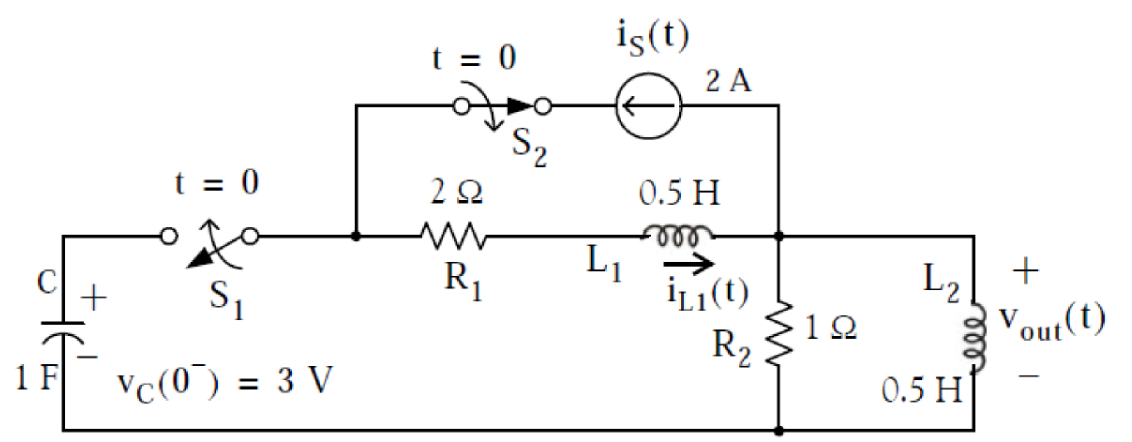
\includegraphics[width=0.95\linewidth]{chrome_p7cOolCXc6.png}
\end{figure}
\vspace{-1em}
\textit{Figure 1}
\end{center}

\item Consider again the circuit in \textit{Fig. 1}. Using the appropriate MATLAB commands, verify that each step of your calculation on paper is correct. Show everything clearly in your report. You may copy and paste your scripts and command window outputs.

\item Plot $v_\text{out}(t)$ for $0 \le t \le 0.05$ s.

\end{enumerate}

\section{Answers}

\begin{enumerate}[leftmargin=*,label=\textbf{\arabic*.}]

\item Investigate the circuit for $t<0$ and $t>0$.

\vspace{1em}

\begin{minipage}{0.47\textwidth}
For $t<0$,
\vspace{-1em}
\begin{center}
\begin{figure}[H]
    \centering
    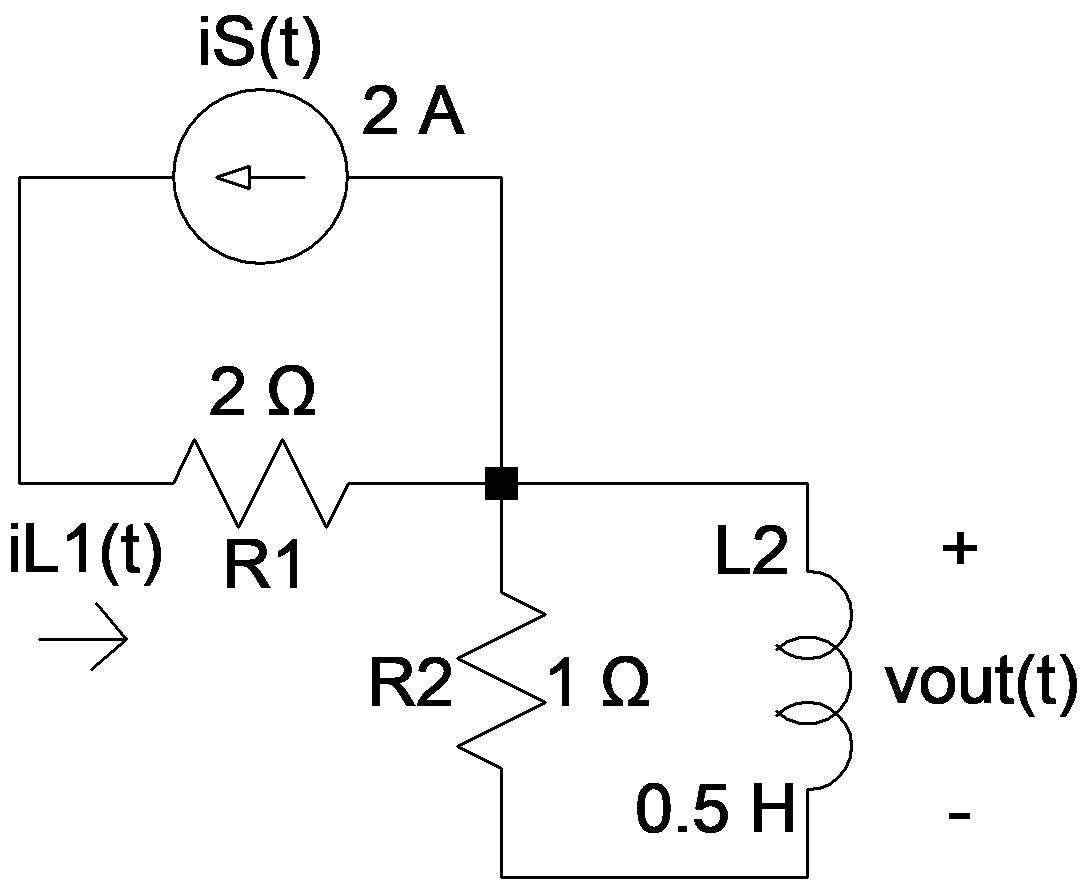
\includegraphics[width=0.85\linewidth]{1.png}
\end{figure}
\vspace{-1em}
\textit{Circuit 2}
\end{center}
\[i_{L_1}(0^-)=2\text{ A}.\]
\end{minipage}\vrule\hfill\begin{minipage}{0.47\textwidth}
For $t>0$,
\vspace{-1em}
\begin{center}
\begin{figure}[H]
    \centering
    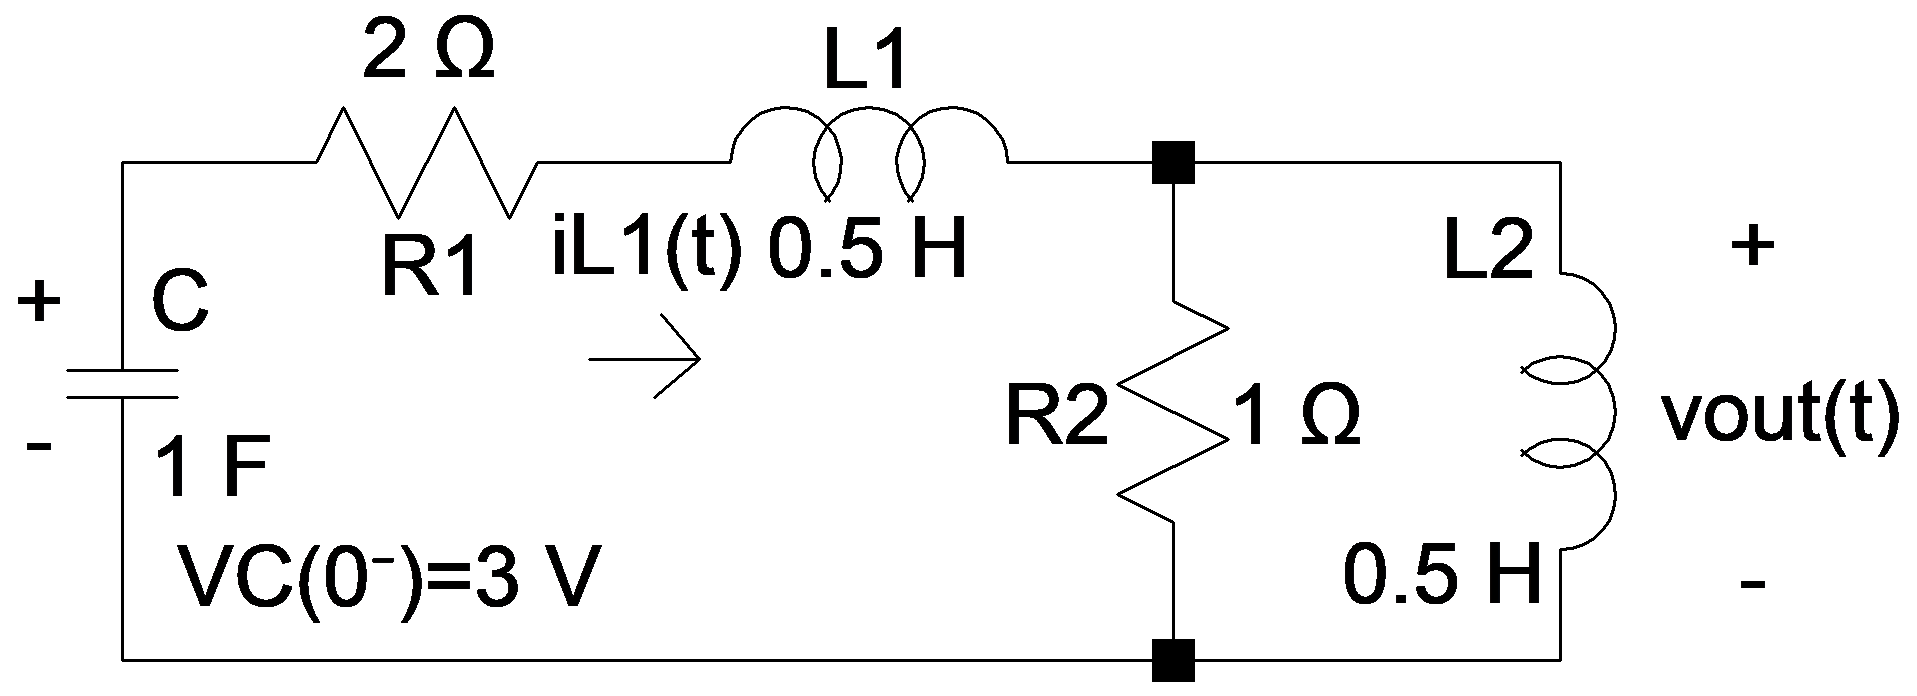
\includegraphics[width=1\linewidth]{2.png}
\end{figure}
\vspace{-1em}
\textit{Circuit 3}
\end{center}
\[i_{L_1}(0)=i_{L_1}(0^-)=2\text{ A}.\]

\vspace{3em}

Transform \textit{Circuit 3} into the $s$--domain as seen below.

\end{minipage}

\vspace{2em}

\begin{center}
\begin{figure}[H]
    \centering
    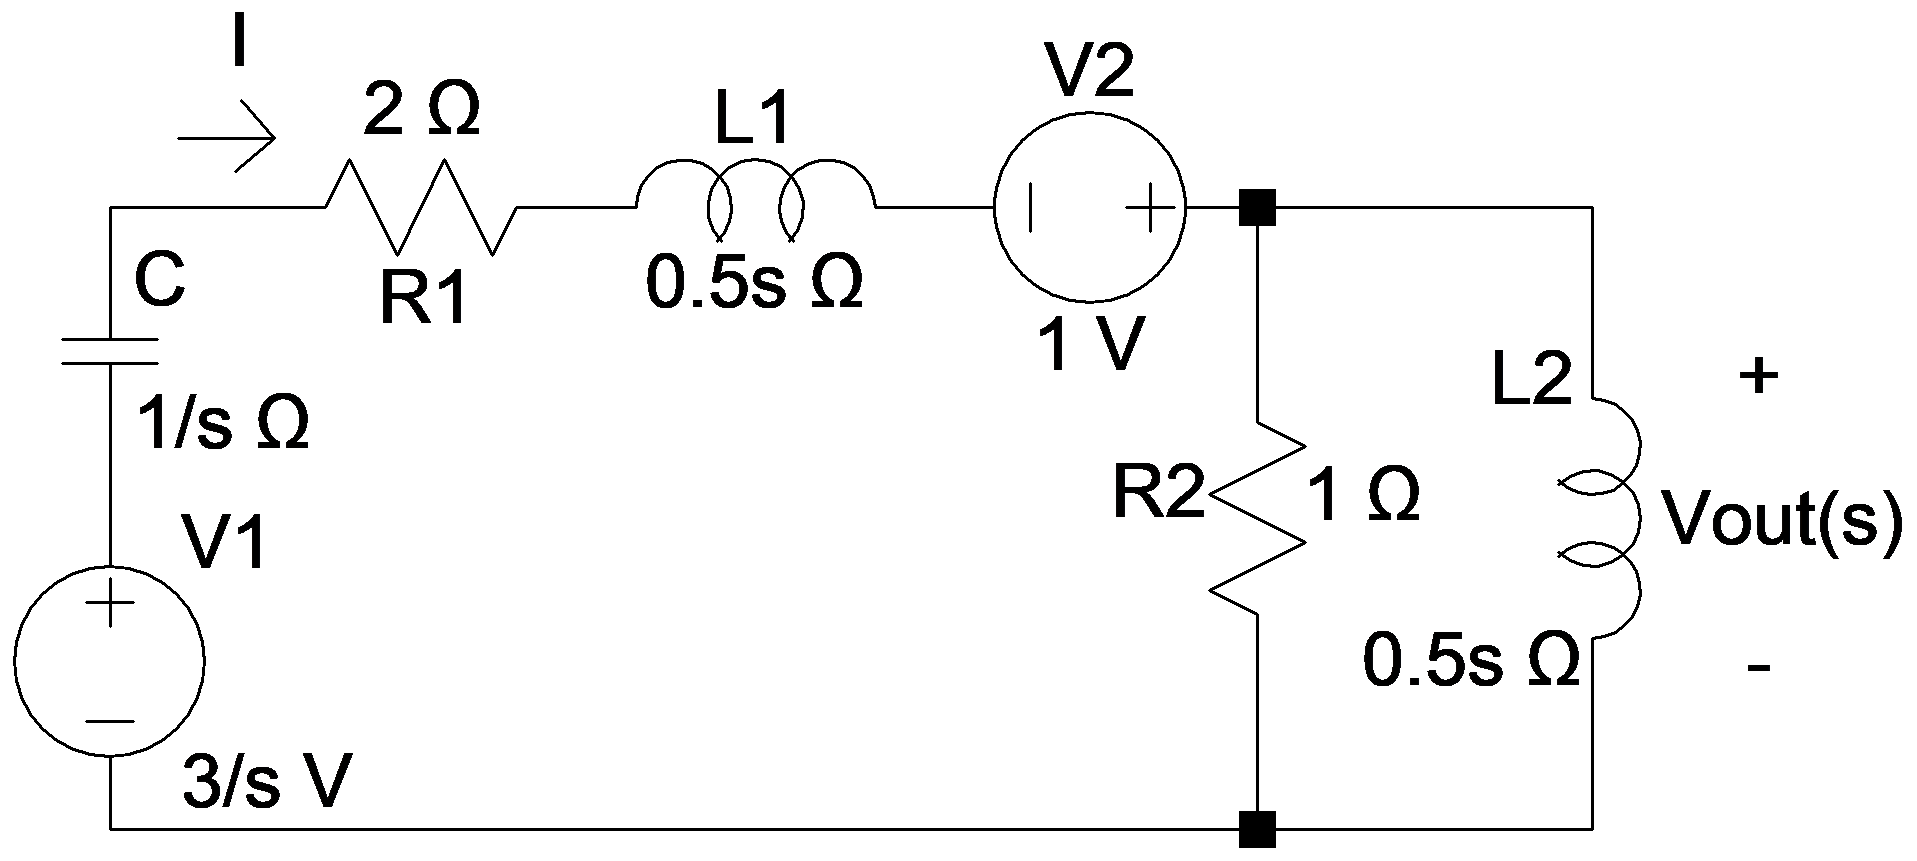
\includegraphics[width=0.6\linewidth]{3.png}
\end{figure}
\vspace{-1em}
\textit{Circuit 4}
\end{center}

\vspace{-1em}

By KVL,
\[-\frac3s+\frac{I(s)}s+2I(s)+0.5sI(s)-1+I(s)\left(\frac{0.5s}{1+0.5s}\right)=0,\]
\[I\left(\frac1s+2+0.5s+\frac{0.5s}{1+0.5s}\right)=\frac3s+1,\]
\[I=\frac{\dfrac3s+1}{\dfrac1s+2+0.5s+\dfrac{s}{2+s}}=\frac{s(2+s)\left(\dfrac3s+1\right)}{s(2+s)\left(\dfrac1s+2+0.5s+\dfrac{s}{2+s}\right)}=\frac{2(s+2)(s+3)}{s^3+8s^2+10s+4}.\]

By the voltage divider,
\[V_\text{out}=I\cdot\frac{1\cdot0.5s}{1+0.5s}=\frac{2s(s+3)}{s^3+8s^2+10s+4}.\]

Find the roots of the expression in the denominator. Numerical approximation gives
\[s_1\approx-6.57,\quad s_2\approx-0.715+j0.313,\quad s_3\approx-0.715-j0.313=s_2^*.\]

Apply partial fraction decomposition.
\[\frac{2s(s+3)}{s^3+8s^2+10s+4}=\frac{A}{s+6.57}+\frac{B}{s+0.715+j0.313}+\frac{C}{s+0.715-j0.313}\]

Find the values $A, B$, and $C$.
\[A=\left.\frac{2s(s+3)}{(s+0.715+j0.313)(s+0.715-j0.313)}\right|_{s=-6.57}\approx1.364\]
\[B=\left.\frac{2s(s+3)}{(s+6.57)(s+0.715-j0.313)}\right|_{s=-0.715-j0.313}\approx0.318-j0.927\approx0.980\,\phase{-71.1^\circ}\]
\[C=\left.\frac{2s(s+3)}{(s+6.57)(s+0.715+j0.313)}\right|_{s=-0.715+j0.313}\approx0.318+j0.927\approx0.980\,\phase{71.1^\circ}\]

Using the inverse Laplace transform table, the solution is then
\[v_\text{out}(t)=\mathcal{L}^{-1}\left\{V_\text{out}(s)\right\}=\left[1.364e^{-6.57t}+1.96e^{-0.715t}\cos(0.313t+71.1^\circ)\right]\cdot u(t).\]

%Solve for $v_{\text{out}}$.
%\[v_{\text{out}}(t)=-\frac1C\int_0^ti_{L_1}(\tau)\,d\tau-R_1\cdot i_{L_1}(t)-L\frac{di_{L_1}}{dt}.\]

%Apply the Laplace transform.
%\[\mathcal{L}\left\{v_{\text{out}}\right\}=\mathcal{L}\left\{-\frac1C\int_0^ti_{L_1}(\tau)\,d\tau-R_1\cdot i_{L_1}(t)-L\frac{di_{L_1}}{dt}\right\}\]
%\[V_{\text{out}}(s)=-\frac1C\frac{I_{L_1}(s)}{s}-R_1\cdot I_{L_1}(s)-L\left(sI_{L_1}(s)-i_{L_1}(0)\right).\]

%Rearranging,
%\[V_{\text{out}}=-I_{L_1}\left(\frac1{Cs}+R_1+Ls\right)=-I_{L_1}\left(\frac1s+2+0.5s\right).\]

%The voltage $V_{\text{out}}$ can be expressed as $V_{\text{out}}=I_{L_1}\cdot\left(\dfrac{1s}{1+0.5s}\right)$. Therefore,
%\[I_{L_1}\cdot\left(\dfrac{1s}{1+0.5s}\right)=-I_{L_1}\left(\frac1s+2+0.5s\right)\implies I_{L_1}=\frac{}{}\]

\newpage

\item Code:

\vspace{1em}

\hrule
\begin{verbatim}
syms s

num = 2*s*(s+3)
denom = s^3 + 8*s^2 + 10*s + 4

Vout = expand(num) / denom

numc = [2 6 0];
denomc = [1 8 10 4];

[r, p, k] = residue(numc, denomc)
\end{verbatim}
\hrule

\begin{figure}[H]
    \centering
    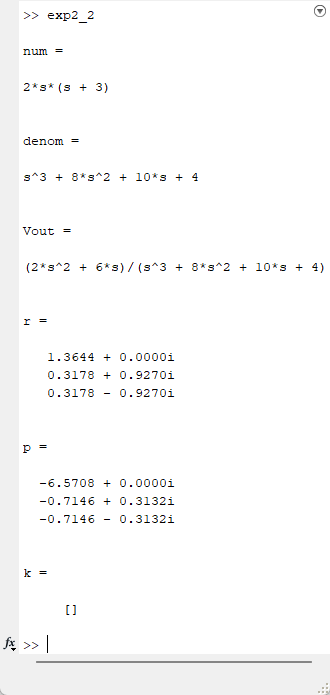
\includegraphics[width=0.5\linewidth]{MATLAB_nOfYrvR8Qa.png}
\end{figure}

We can infer from the command window that the values are consistent.
\newpage

\item Code:

\vspace{1em}

\hrule
\begin{verbatim}
set(gca,'TickLabelInterpreter','latex')

t = 0:0.0001:0.05;
Vout = 1.36*exp(-6.57*t) + 1.96*exp(-0.715*t).*cos(0.313*t+degtorad(71.1));
plot(t, Vout)

grid on

xlabel('$t$', Interpreter='latex')
ylabel('$V_{\textrm{out}}$', Interpreter='latex')
title('Graph: $V_{\textrm{out}}$ over time', Interpreter='latex')
\end{verbatim}
\hrule

\begin{figure}[H]
    \centering
    
\includegraphics[width=0.85\linewidth]{fig1.png}
\end{figure}

\end{enumerate}

\end{document}